\section{Witness Implementation} \label{section:witness-implementation}
With the extended Raft algorithm, the witness possesses the following properties that make it particularly suitable for implementation as a storage object:

\begin{itemize} 
    \item Witness does not have volatile variables, implying that all states within the witness are persisted in durable storage. 
    \item Witness only persists a small amount of metadata. Neither user data nor the full log prefix metadata are stored in witness. This results in a trivial and predictable capacity requirement. 
    \item Witness is rarely accessed. The shortcut replication ensures that leader only needs to write to witness when its replication set changes. Therefore, witness may only need to be accessed when faults change (e.g. a server shuts down or recovers) or a candidate requests its vote. In a relatively stable cluster, neither of these events occur frequently. 
\end{itemize}

The absence of volatile variables allows the synchronization of witness states to be distributed across all regular servers. For each log replication between leader and witness, the $HandleAppendEntriesToWitnessRequest$ action can be implemented in the leader as a single operation that loads states from the witness's durable storage, make new states according to $HandleAppendEntriesToWitnessRequest$, and writes back new states to the witness's durable storage. Similarly for voting between candidate and witness, the $HandleRequestWitnessVoteRequest$ action can be implemented in the candidate as a single operation that loads states from the witness's durable storage, make new states according to $HandleRequestVoteToWitness$, and writes back the new states to the witness's durable storage. These two implementations can be synchronized using an optimistic concurrency control scheme since they both occur infrequently.

Figure \ref{fig:share-witness-implementation} illustrates an implementation using a share (NFS or SMB) as a witness. We associate a version number with the states, starting from 0. Each modification to the states increases the version by 1. We can then persist each version of the witness states in a file uniquely named after the version number (e.g. \textless{}version\textgreater{}.st). Whenever $HandleAppendEntriesToWitnessRequest$ or $HandleRequestVoteToWitness$ are invoked, a regular server (leader or candidate) loads the witness states from the file with the largest version number, calculates the new states, and saves the new states back to a distinct temporary file (e.g. \textless{}server id\textgreater{}.\textless{}version\textgreater{}.st). Then, the regular server tries to create a hard link from the temporary file to the desired versioned state file (i.e. \textless{}version+1\textgreater{}.st). As long as the file system guarantees atomicity in creating hardlinked files, the regular server will only succeed if the target versioned state file does not exist. If any other server has finished update states in the same version, the process needs to be repeated from the beginning. The optimistic concurrency control eliminates the need for locking overhead, which is challenging to implement in practical applications. The infrequency of witness visits makes such a scheme very suitable.

\begin{figure}
    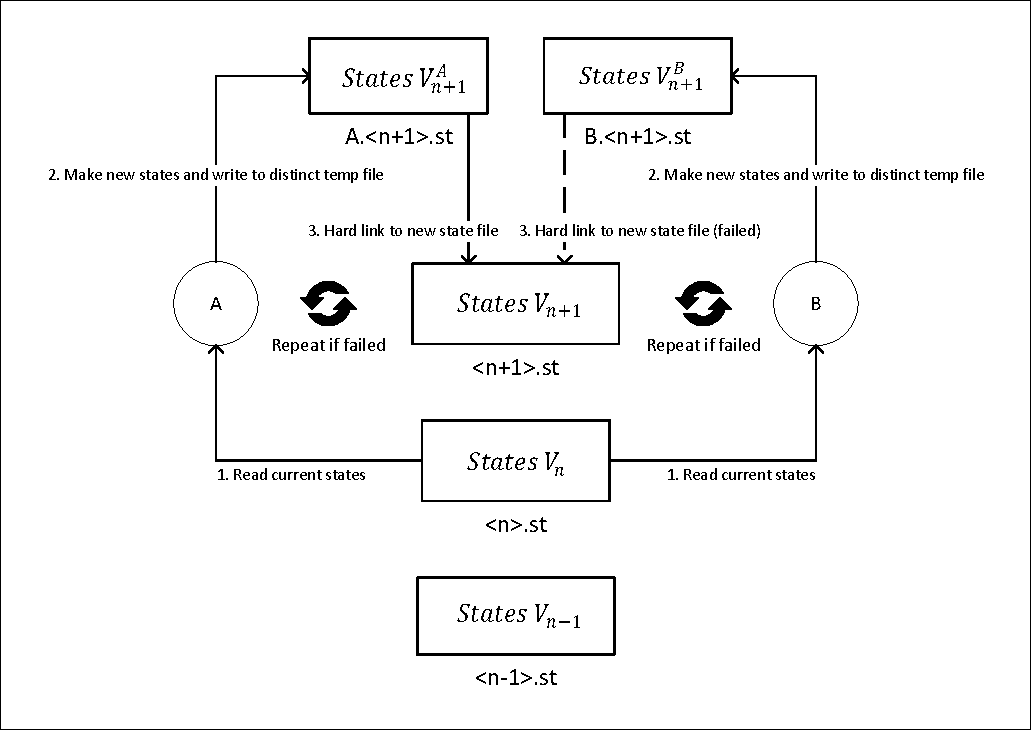
\includegraphics[width=1\textwidth, angle=0]{share-witness-implementation.pdf}
    \caption{Implement witness as a share}
    \label{fig:share-witness-implementation}
\end{figure}

In addition to share, the witness functionality can also be incorporated into cloud storage, such as Azure Storage or AWS S3. Many cloud storage vendors provide optimistic concurrency mechanism for updating object data. For instance, Azure Blob Storage allows clients to update a blob object using the original ETag, combined with a conditional header, to ensure that updates only occur if the ETag remains unchanged. This guarantees that no other client has updated the blob object concurrently. The infrequent access requirements and trivial payload size for witness make cloud storage an ideal solution for this function. Consequently, it provides a broader range of implementation options for end-users.